% Chapter 3

\chapter{The COMPASS experiment at CERN} % Chapter title

\label{ch:exp} % For referencing the chapter elsewhere, use \autoref{ch:name}

In this chapter a description of the COMPASS experiment is provided. The general features of the spectrometer are given in Section~\ref{sec:specgen}. The beam and target are presented in Section~\ref{sec:beam}. The descriptions of the detectors used for the tracking and the ones used for the particle identification are done in Section~\ref{sec:track}, respectively. The trigger system is discussed in Section~\ref{sec:trigger}. The last sections describe data acquisition and reconstruction.

%----------------------------------------------------------------------------------------

\section{General Overview}\label{sec:specgen}

COMPASS is a high energy, high rate fixed-target experiment at the Super Proton Synchrotron (SPS) at CERN. It is dedicated to the study of hadron structure and hadron spectroscopy with high intensity muon and hadron beams.

In order to cover the necessary large range in $Q^2$ and $x$ for the available beam energy the COMPASS spectrometer as shown in Fig.~\ref{pic:apparatus} covers a large momentum and angular range. This is obtained by usinf a two-stage spectrometer for detecting outgoing particles.

The apparatus is divided in three parts: the first part is dedicated to the detection of the incoming beam and is located upstream the target location. The second and third part are located downstream of the target and represent a length of $50$ meters. The second part called the \textit{Large Angle Spectrometer} (LAS) is built around the magnet SM$1$. The LAS has been designed to provide a $180$ mrad acceptance. The \textit{Small Angle Spectrometer} (SAS), built around the magnet SM$2$, measures the particles emitted at small angles ($\pm$ $30$ mrad).

In $2016$, the data taking was performed with a $160$ Gev/c muon beam scattering off a liquid H$_2$ target.

\begin{sidewaysfigure}[!p]
  \centering
	\subfloat[LAS]{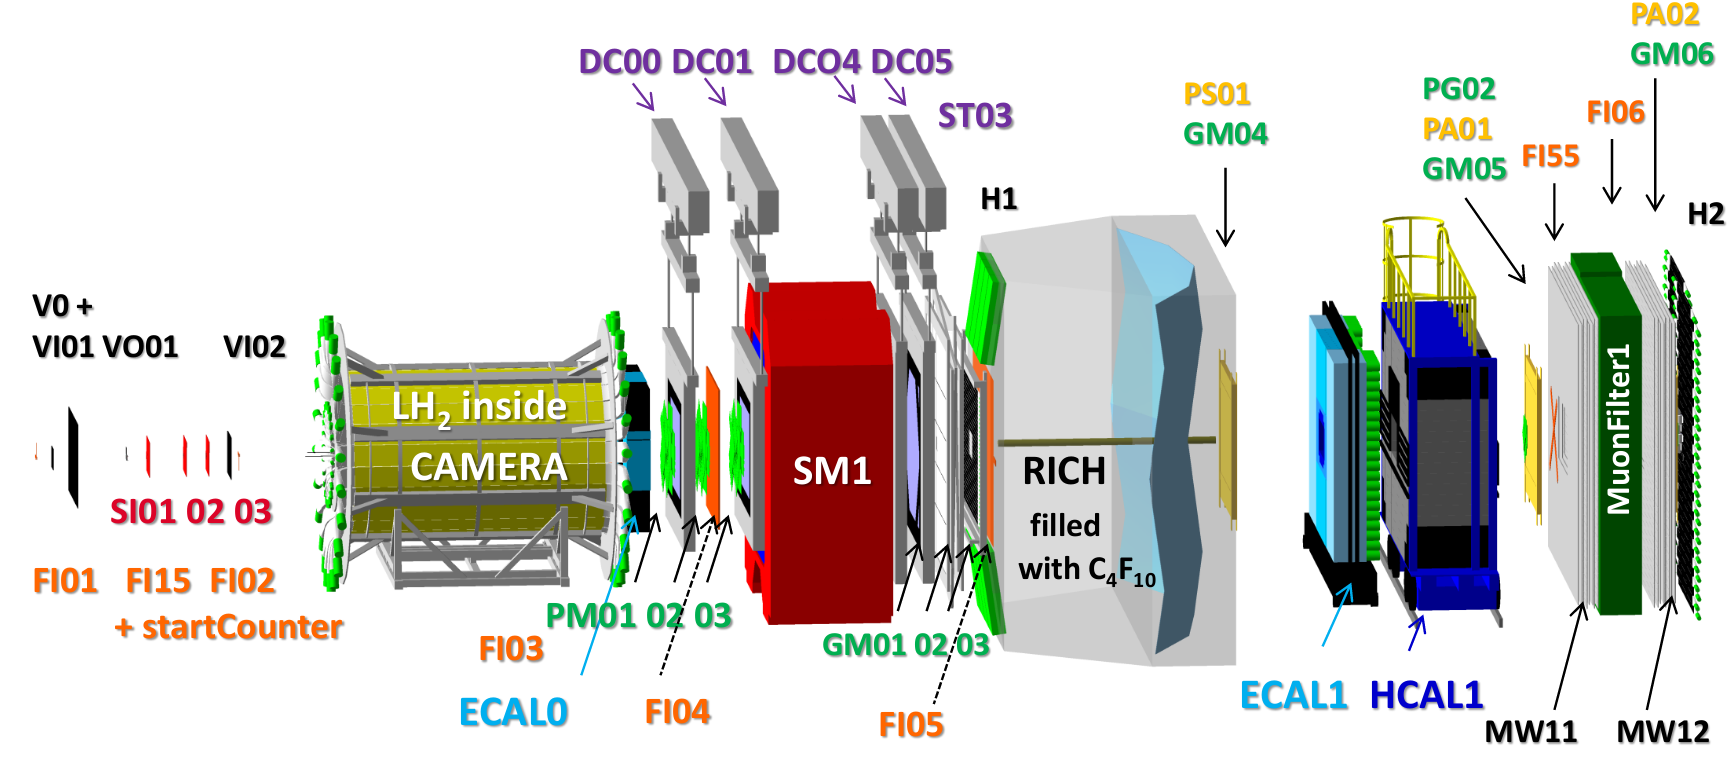
\includegraphics[scale=0.28]{./gfx/Apparatus1.png}}
  \subfloat[SAS]{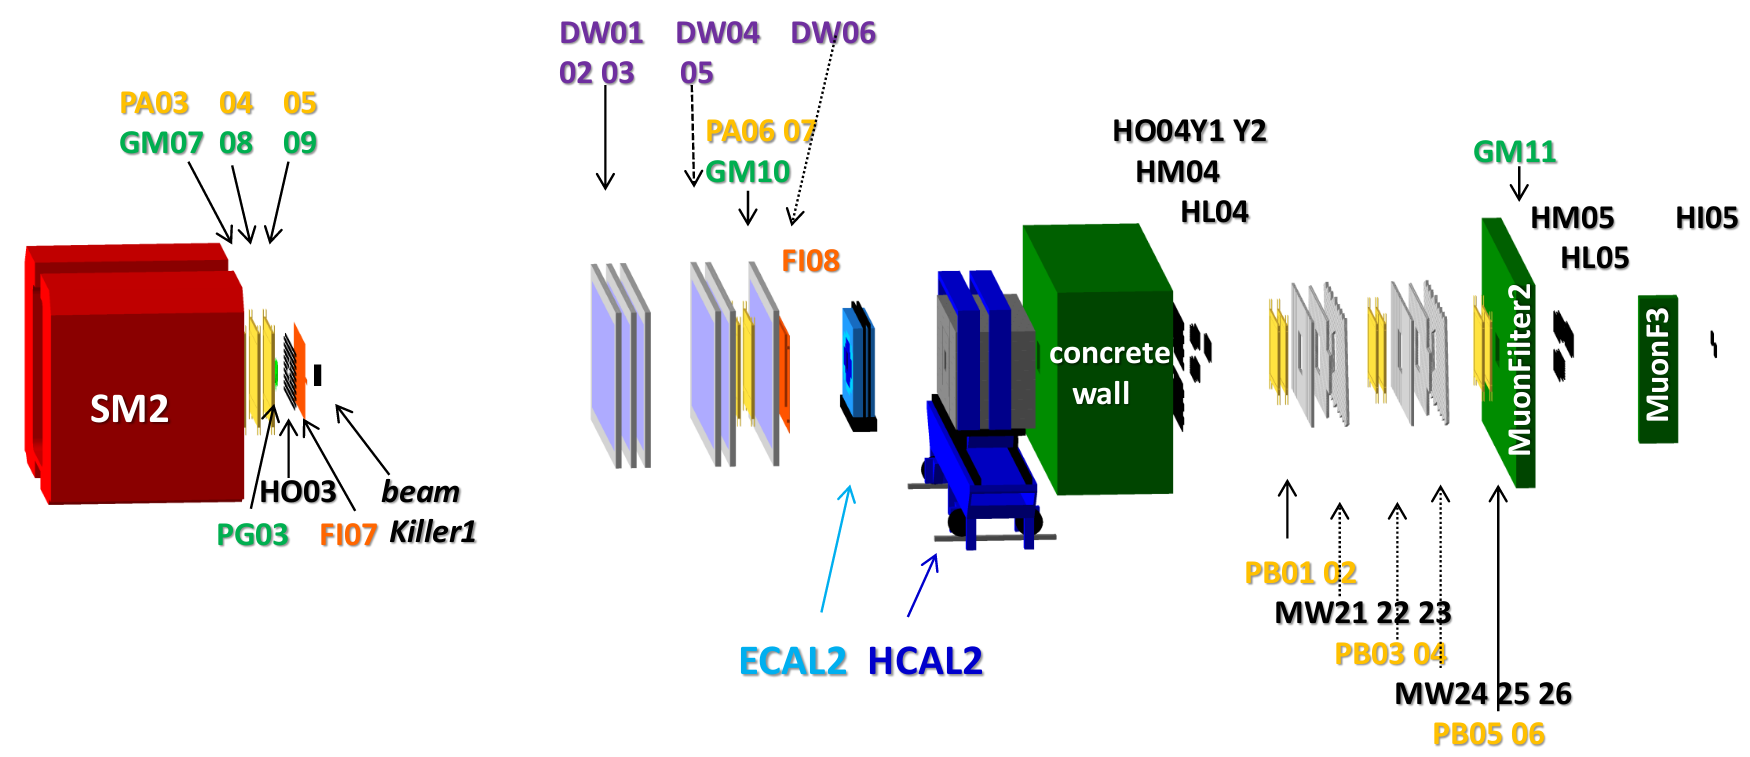
\includegraphics[scale=0.28]{./gfx/Apparatus2.png}}
	\caption{COMPASS 2016/2017 muon setup side view. The two stages of the spectrometer at different scales in this drawing. Taken from \cite{Setup}.}
	\label{pic:apparatus}
\end{sidewaysfigure}

%----------------------------------------------------------------------------------------

\section{Beam}\label{sec:beam}

The muon beam used by COMPASS is obtained from a primary proton beam accelerated in the SPS to $400$ GeV/c. The proton beam interacts with T6 target, a $50$ cm thick beryllium target, producing mainly pions and kaons. The spill time, which is the time window, within which the proton beam is delivered to the T6 target, was of $4.8$ s. In each cycle of $36$ s there were two spills.

\subsection{The M$2$ Beam Line}

The hadrons produced at T$6$ are transported in the $600$ m long decay channel of the M$2$ beamline \cite{NIM2015,M2Beam}. During this time, $5$\% of the pions and kaons are decaying into muons and neutrinos. At the end of this $600$ m decay section, the remaining hadrons are stopped by a hadron absorber and the muons are focused. A system of magnets is then used to select and focus the muons of $160$ GeV/c.

The beam has transverse dimensions of $\sigma_x \times \sigma_y \sim 8 \times 8 $ mm$^2$ and an angular divergence of $\sigma_{\theta_x} \times \sigma_{\theta_y} \sim 0.5 \times 1 $ mrad$^2$ in the experimental area. At each spill, $2\cdot10^8$ muons enter the experimental area. The beam is accompanied by a muon halo that extends transversely up to several meters of distance with respect to the beam line. The intensity of this halo decreases with the distance. The halo near the beam line as measured by a $30 \times 30$ cm$^2$ dedicated veto counter with a 4 cm diameter central hole represents about $16$\% of the muon beam. The far halo or low intensity halo is measured by a large veto counter with a central hole of $30 \times 30$ cm$^2$. It represents about $7$\% of the muon beam.

\subsection{The Beam Momentum Station}

The Beam Momentum Station (BMS) illustrated in Fig.~\ref{pic:BMS} is used for the determination of the incident muon momentum. It consists of six scintillators hodoscopes (BM$01$-BM$06$) located asymmetrically upstream and downstream a bending magnet (B$6$: three consecutive dipole magnets) surrounded by four quadrupoles (Q$29$-Q$32$).

The BMS system was designed to measure the momentum of more than $10^8$ individual particles per spill with a relative precision of $0.5$\%. To eliminate the ambiguities in the reconstruction of particle trajectories, their time of transit is measured with a resolution of $50$~ps.

\begin{figure}[!h]
  \centering
	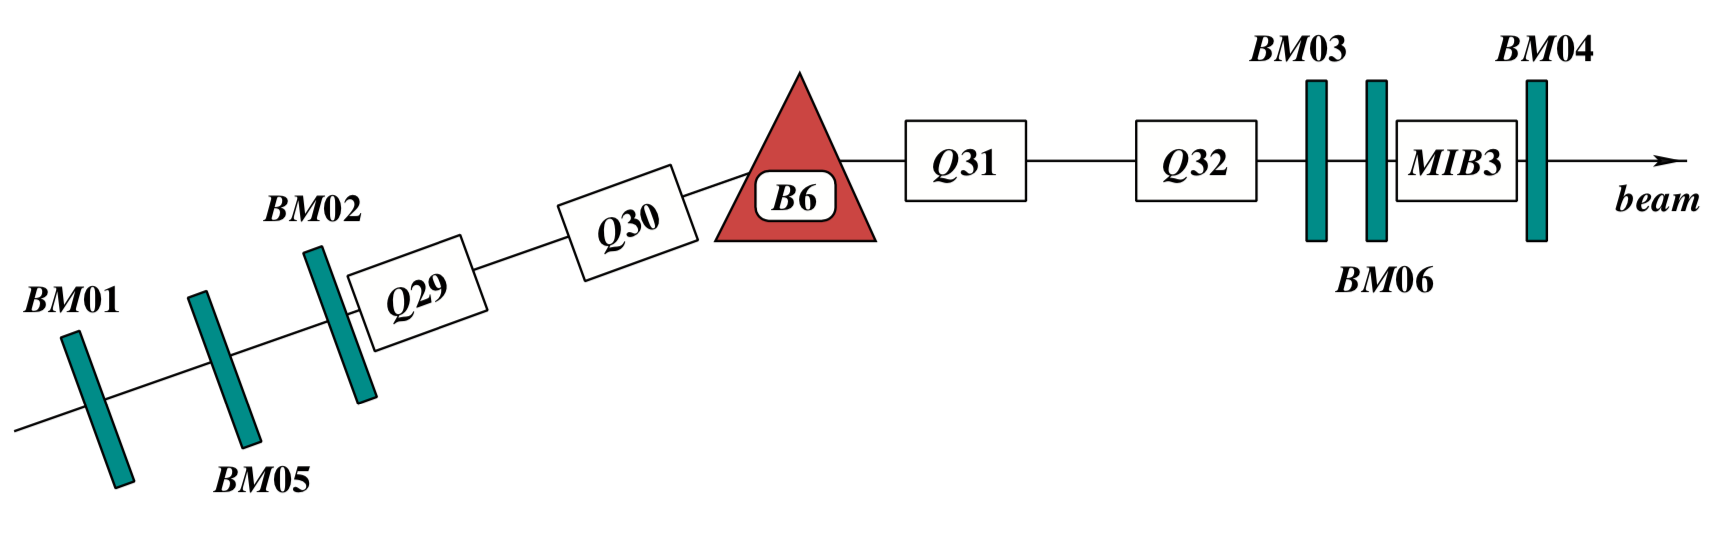
\includegraphics[scale=0.5]{./gfx/BMS.png}
	\caption{Layout of the Beam Momentum Station for the COMPASS muon beam. Taken from \cite{NIM}.}
	\label{pic:BMS}
\end{figure}

%----------------------------------------------------------------------------------------

\section{Target}

\begin{figure}[!h]
  \centering
	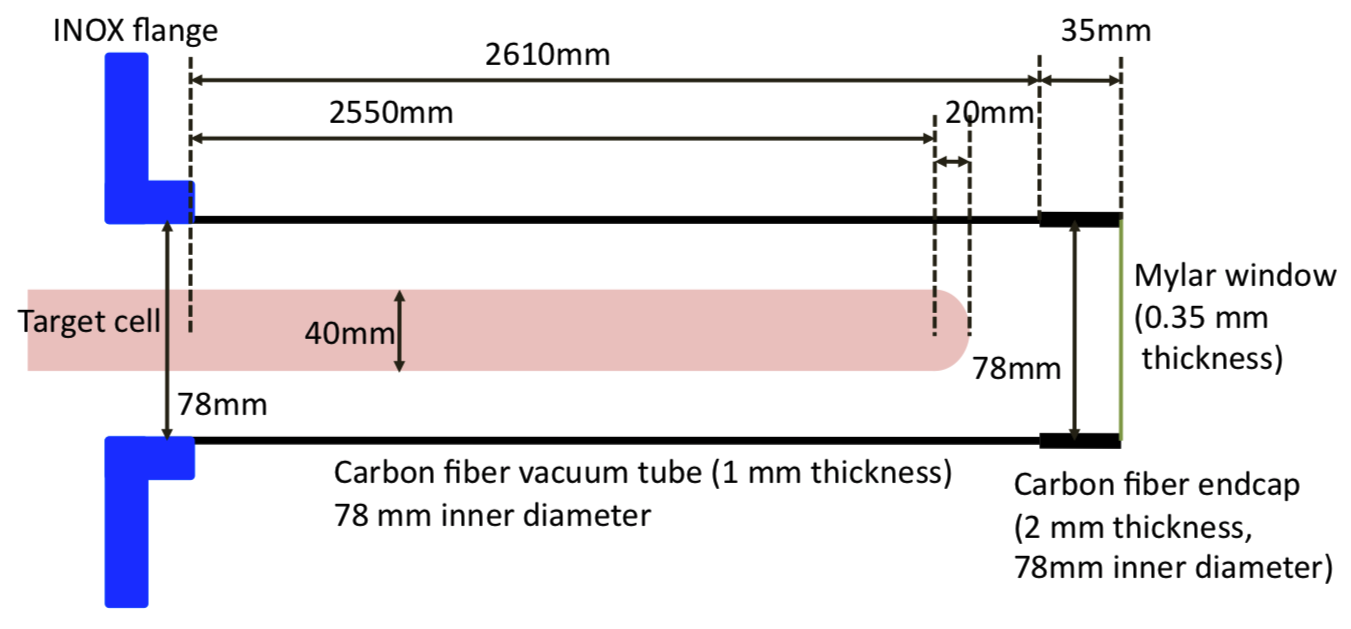
\includegraphics[scale=0.3]{./gfx/Target.png}
	\caption{Target geometry for the 2016/2017 setup.}
	\label{pic:TargetSetup}
\end{figure}

The target is liquid $H_2$ contained in a $2.5$ meter long cylinder (Fig. \ref{pic:TargetSetup}). The target material is contained in a mylar tube with a diameter of $4$ cm. The total volume of the target cell and the liquid hydrogen system is located in a cryostat made of carbon fiber. The operation temperature of hydrogen is $18$ K with a pressure of $1020$~mbar. The material for the target cell was chosen in order to minimise proton absorption.

%----------------------------------------------------------------------------------------

\section{Tracking Detectors}\label{sec:track}

The \textit{Large Angle Spectrometer} (LAS) and \textit{Small Angle Spectrometer} (SAS) are each equipped with different type of tracking detectors. Depending on the direction coverage area of each detectors they are classified as:
\textit{very small area trackers}, \textit{small area trackers} and \textit{large area trakers}

\subsection{Very small area trackers}

The very small area trackers cover the transverse beam size up to $\sim$ $3$ cm. In this region the particle rate is very high ($10^5$/s/mm$^2$ in the center of the muon beam), hence the tracking detectors must have an excellent time and position resolutions.

The scintillating fibre detectors are used at several locations of the experiment and cover areas between $\sim$ $16$ cm$^2$ and $144$ cm$^2$. They are fabricated from $0.5$-$1$ mm diameter fibres and reach a time resolution better than $500$ ps. All along the apparatus there are $9$ stations composed by two or three scintillating fiber detectors. The third detector is always pivoted by $45$° with respect to the others.

The silicon detector size is $5$x$7$ cm$^2$ with a space and time resolution of $\sim$ $10$ $\mu$m and $<$~$2.5$~ns. The $3$ silicon detectors stations are located upstream the target. The stations are each composed by two silicon detectors, the second one being rotated by $5$° with respect to the other, each detector measuring perpendicular views.

\subsection{Small area trackers}

The radial region between $2.5$ cm and $20$ cm is covered by two types of gaseous detectors~: PixelMicromegas (MICRO MEsh GAseous Structure) and (Pixel)GEM (Gas Electron Multiplier) detectors. These detector have a high rate capability ($\sim$ $10^4$/s/mm$^2$) and good spatial resolution ($<$ $100$ $\mu$m). They also present a minimal material budget.

The principle of the PixelMicromegas is explained in Fig.~\ref{pic:MM} (a). The particle ionizes the gas in the conversion gap, the produced electrons drift in a moderate field of $1.5$ kV/cm to prevent secondary ionization, towards the amplification gap. The field in the amplification area is large enough to accelerate the electrons to produce an avalanche. The conversion and amplification gaps are separated by a \textit{micromesh}, which collects the positive ions produced during the avalanche in a short period of time ($<$ $100$ ns). This feature is possible because of the small width of the gap ($\sim$ $100$ $\mu$m). The PixelMicromegas have an active area of $40 \times 40$ cm$^2$ with a central area made of 1280 pixels of $400$ $\mu$ m $\times$ $2.5$ mm and $400$ $\mu$ m $\times$ $6.5$ \cite{FloThi} as shown in Fig.~\ref{pic:MM} (b). All PixelMicromegas detectors operate with a detection efficiency of $98$\% and with a spatial resolution of better than $100$ $\mu$m. There are three PixelMicromegas stations located at LAS. They are composed by four detectors each with different directions: horizontal (X), vertical (Y), and two (U,V) rotated by $\pm$ $45$° with respect to the vertical. Each plane has an active area of $40 \times 40$ cm$^2$.

\begin{figure}[!h]
  \centering
	\subfloat[]{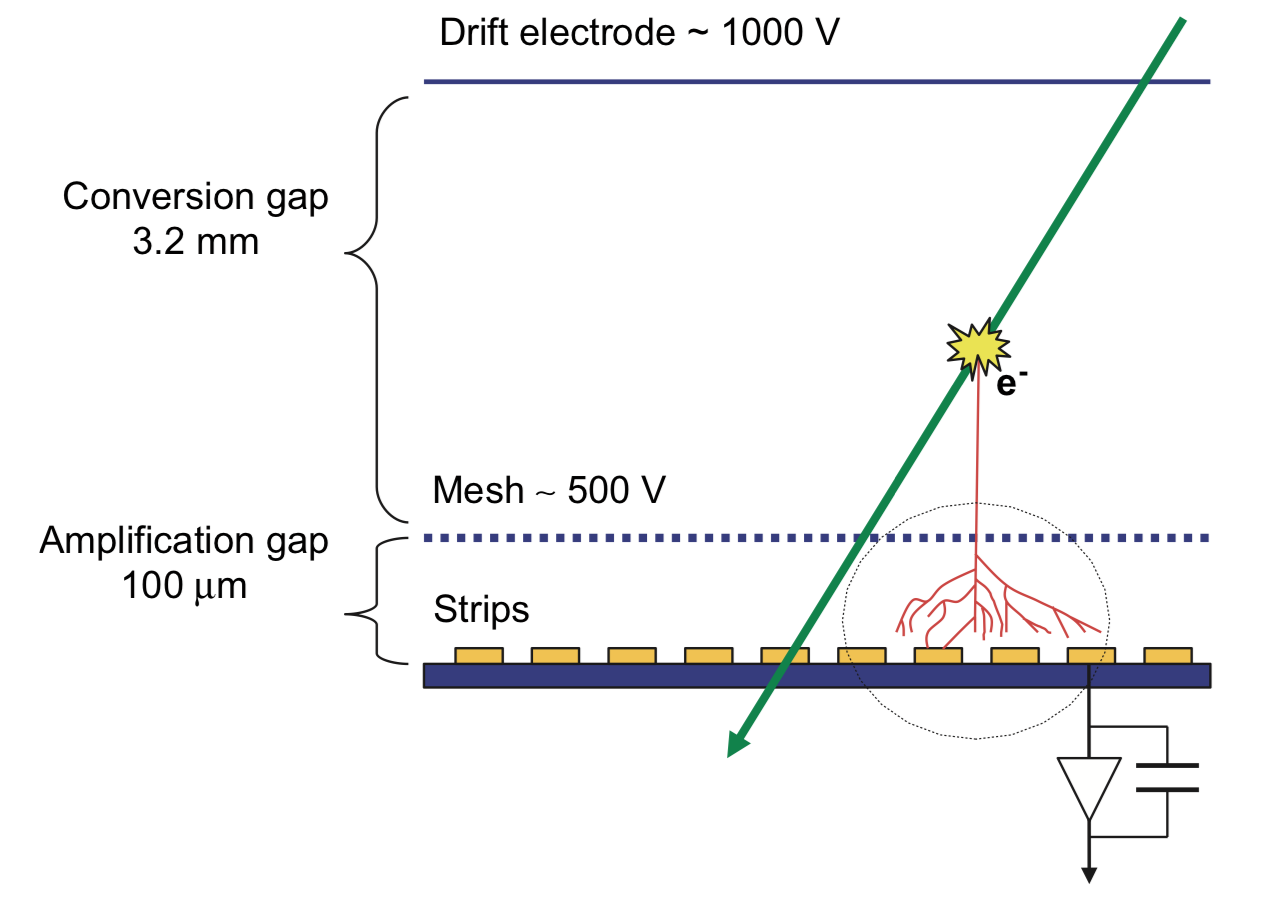
\includegraphics[scale=0.35]{./gfx/MM1.png}}
  \subfloat[]{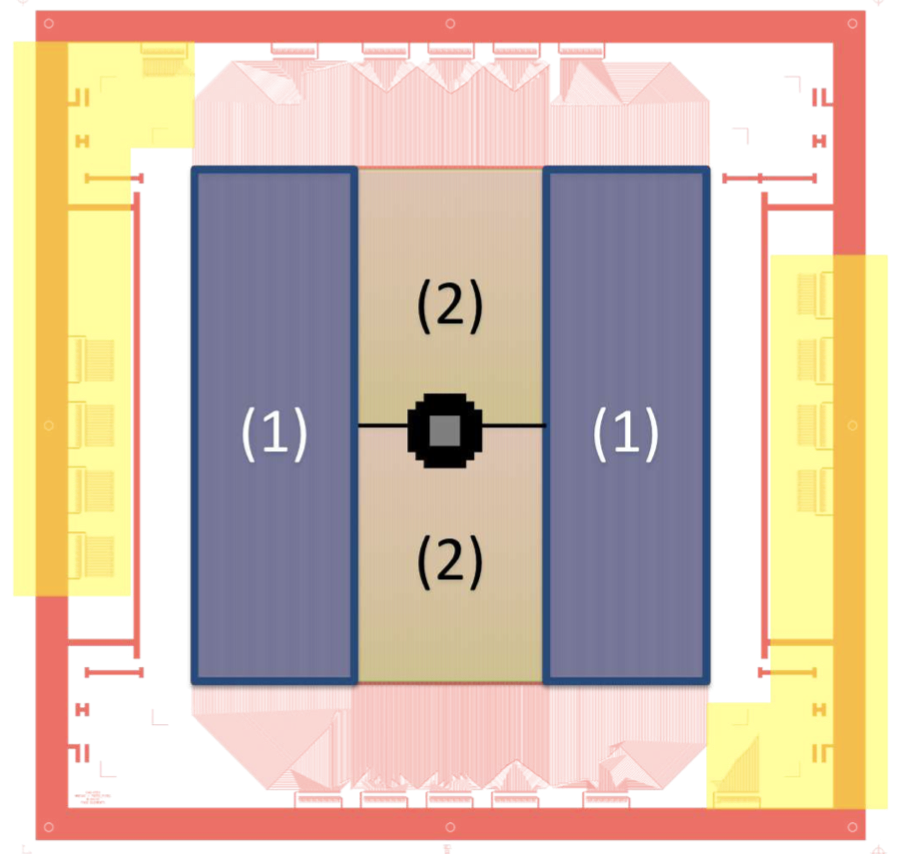
\includegraphics[scale=0.35]{./gfx/MM2.png}}
	\caption{(a) COMPASS MicroMegas detection principle. Taken from \cite{NIM}. (b) PixelMicromegas detector geometry. (1) Tracks of $40$ cm $\times$ $480$ $\mu$m; (2) Tracks of $20$ cm $\times$ $400$ $\mu$m; In the center is the pixellized area. Taken from \cite{FloThi}.}
	\label{pic:MM}
\end{figure}

A GEM is a $50$ $\mu$m thin polyimide foil with Cu cladding on both sides, into which numerous microholes ($\sim$ $10^4$/cm$^2$) with a diameter of $70$ $\mu$m have been chemically etched using lithographic techniques. A high voltage (several $100$ V) is applied between the surfaces of the foil to generate the avalanche multiplication of electrons through the holes. The fast signal is induced by the electron cloud emerging from the last GEM foil on an anode segmented into two sets of $768$ orthogonal strips (pitch of $400$ $\mu$m). The COMPASS GEM detection principle is shown in Fig.~\ref{pic:GEM}: it consists of three GEM amplification stages separated by thin grids of $2$ mm height (transfer gap). Using several GEMs in a stack allows to split the gas gain over several GEMs and reduce the voltage across the two sides of the used GEM foils thus achieving the same gain while reducing the probability for discharges. The COMPASS PixelGEM are GEMs with a pixellized central area. A GEM station is composed by $2$ detectors oriented by $45$° relatively to each other. All in all there are $11$ GEM stations and $2$ PixelGEM stations located after SM$1$ and at SAS. The active area for the GEM is $31 \times 31$ cm$^2$ and the central area of $5$ cm diameter can be activated to align the detector with low intensity beams. The PixelGEM have an active area of $10 \times 10$ cm$^2$ with a central area of $3.2 \times 3.2$ cm$^2$ filled with $1$ mm$^2$ squared pixels. The detectors efficiency is $\sim$ $97$\% with a spatial and time resolution of about $\sim$ $70$ $\mu$m and $12$ ns, respectively.

\begin{figure}[!h]
  \centering
	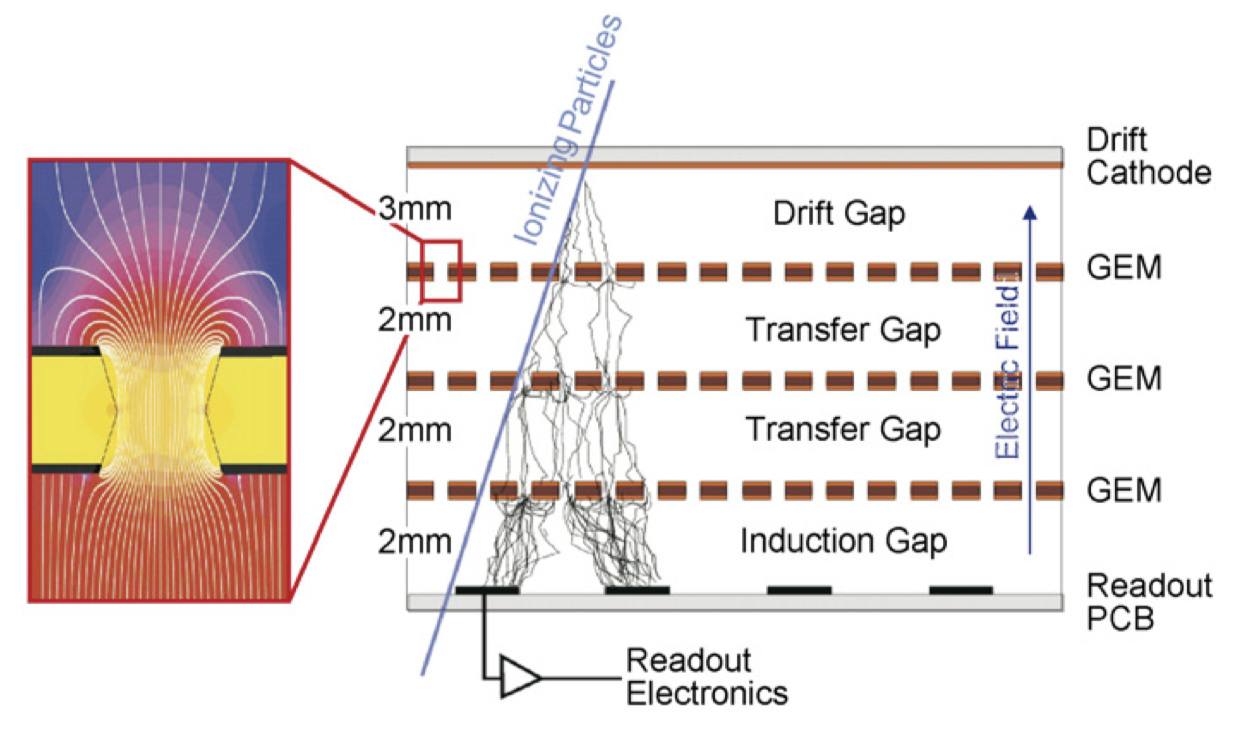
\includegraphics[scale=0.5]{./gfx/GEM.png}
	\caption{COMPASS GEM detection principle. Taken from \cite{NIM}.}
	\label{pic:GEM}
\end{figure}

\subsection{Large area trackers}

The large area trackers cover all the remaining spectrometer acceptance with a good spatial resolution. As the particle rate in the region covered by the large area trackers is small in comparison to the central region ($10^2$/s/mm$^2$), the use of detectors such as drift chambers (DCs and W$4/5$) \cite{DaCosta}, straw drift tubes \cite{Zvyagin} and multiwire proportional chambers (MWPCs) is possible. These detectors have large active size area ($\sim$ m$^2$) with a central dead area of few cm$^2$.

Each DC consists of eight layers of wires with four different inclinations: horizontal, vertical and rotated $\pm$ $20$° with respect to the vertical direction (X, Y, U and V). Two consecutive planes with the same inclination are staggered by $3.5$ mm to disimbiguate left-right and the ordering of the planes with different orientations is such to minimize the fake track combinations. The detectors are filled with a gas mixture of Ar, C$_2$H$_6$ and CF$_4$ at a volume ratio $9:9:2$. Two of the DC are located before SM$1$ and have an active area of $180 \times 127$ cm$^2$~. the last two are located downstream SM$1$ and have a larger active area of $204 \times 204$ cm $^2$. All these DCs have a central dead area of $30$ cm. The central dead area can be activated for alignment needs with a low intensity beam. The average resolution of a DC is $270$ $\mu$m and the efficiency above $95$\%.

The W$4/5$ detectors have an active area of $5$ x $2.5$ m$^2$, and consist of $4$ anode wire layers with a wire pitch of $4$ cm. The anode wires are separated by layers of cathode wires with a pitch of $2$ mm. The diameter of the anode wire is $20$ $\mu$m and of the potential wires, $200$ $\mu$m. A CF$_4$-based gas mixture, Ar/CF$_4$/CO$_2$ ($85/10/5$), is used.

A straw detector station consists in $3$ straw detectors with different orientations: horizontal, vertical and rotation by $10$° with respect to the vertical. The only station used is located between SM$1$ and SM$2$. Each detector is composed by two layers of straw tubes with the same orientation. The straw tubes consist in two layers of thin plastic film, one coated with carbon loaded Kapton, the other one with aluminised Kapton foil. The active area for the straw detector is $320 \times 280$ cm$^2$ and have a central dead area of $20 \times 20$ cm. The average resolution is of $190$ $\mu$m.

There are three types of MWPCs in COMPASS, which differ by the number of layers, the size of the dead area for the beam and the combination of the measured projections (X, Y, U and V). The active area is of $178 \times (90-180)$ cm$^2$. All layers have a wire length of about $1$ m, a wire diameter of $20$ $\mu$m and a pitch of $2$ mm and are enclosed on both sides by graphite-coated Mylar foils. The central deadarea of each detector increases with respect to the detector position, from $16$ to $22$ cm. The average spatial resolution of the MWPC is of $1.6$ mm.

\begin{table}[!h]
  \caption{Table with the characteristics of a selection of tracking detectors.}
  \label{tab:kinvar}
  \centering
  \begin{tabular}{c|c|c|c}
    \hline
    \hline
    Detector type & Active area & Spacial resolution & Time resolution \\
    \hline
    \hline
    Scintillating Fibre & $(3.9)^2$ - $(12.3)^2$ cm$^2$ & $130$ - $210$ $\mu$m & $400$ ps \\
    Silicon Micro-strip & $5$ x $7$ cm$^2$ & $8$ - $11$ $\mu$m & $2.5$ ns \\
    (Pixel)GEM & $31$ x $31$ cm$^2$ & $70$ $\mu$m & $12$ ns \\
    PixelMicromegas & $40$ x $40$ cm$^2$ & $90$ $\mu$m & $9$ ns \\
    MWPC & $178$ - $(90-120)$ cm$^2$ & $1.6$ $\mu$m & N/A \\
    DC & $180$ - $127$ cm$^2$ & $190$ - $500$ $\mu$m & N/A \\
    Straws & $280$ - $323$ cm$^2$ & $190$ $\mu$m & N/A \\
    \hline
    \hline
  \end{tabular}
\end{table}

%----------------------------------------------------------------------------------------

\section{Particle Identification}

Following the nature of the particles, several techniques are used to identify them. Two types of calorimeters are used to measure the energy of the hadrons, photons and electrons: hadron calorimeters (HCAL$1$ and HCAL$2$) separate hadrons and muons and electromagnetic calorimeters (ECAL$0$, ECAL$1$ and ECAL$2$) detect and identify photons. Two muon wall detectors (MW$1$ and MW$2$) are used together with a hadron absorber for muon identification (muon filter). A RICH detector allows to separate between pions, kaons and protons in the momentum range from $3$ to $50$ GeV. While the RICH will be further described in a dedicated chapter (Chapter~\ref{ch:PID}), the other identification detectors will be briefly described in the following subsections.

\subsection{Hadron Calorimeters}

A hadron calorimeter allows to separate hadron and muon tracks using the energy deposit. Contrary to a hadron, which deposits almost all its energy via a hadron shower, the muon suffers energy loss only depositing a small energy fraction. HCAL$1$ and HCAL$2$ are sampling calorimeters with a modular structure with iron and scintillator plates and are located before the muon filters. Their threshold depends on the energies: for HCAL$1$ for hadrons with momenta above $5$ GeV/$c$ it is almost constant and close to $100$\% when for HCAL$2$ the same efficiency is reached for hadrons with momenta above $10$ GeV/$c$.

\subsection{Electromagnetic Calorimeters}

The electromagnetic calorimeters are used to measure the energy of electrons and photons. ECAL$0$ is made of radiation-hard Shashlyk-type lead/scintillator modules. ECAL$1$ and ECAL$2$ are formed by blocks of lead glass connected to photomultipliers with light guides. An electromagnetic shower is initiated when the incoming electrons or photon reach the calorimeter. This electromagnetic shower produces Cherenkov radiation inside the lead glass and this light intensity is proportional to the energy deposited. The inner-most part of ECAL$2$ has Shashlyk modules.

\subsection{Muon Identification with Muon Walls and Muon Filters}

An efficient way to identify muons is to use an absorber surrounded by two tracking detec- tors. With a radiation length large enough to absorb all hadrons, particles detected behind the absorber are considered muons. At COMPASS, this is done in the LAS with the Muon Wall $1$ (MW$1$) and the Muon Filter $1$ (MF$1$). In the SAS, the Muon Wall $2$ (MW$2$) in combination with the Muon Filter $2$ (MF$2$) identify the muons. At the very end of the spectrometer, the Muon Filter $3$ (MF$3$) is the last muon filter detector. The three muon filters are made of iron or concrete. The MW$1$ system consists of Mini Drift Tubes. The tubes are made of $0.6$ mm thick aluminum tubes surrounding a $50$ $\mu$m thick tungsten wire. The muon filter surrounded by the MW$1$ system is made of $60$ cm of iron. The active areas are $4845$ x $4050$ mm$^2$ (hole: $1445$ x $880$ mm$^2$) and $4730$ x $4165$ mm$^2$ (hole: $1475$ x $765$ mm$^2$) for the X and Y planes. The gas mixture of MW$1$ is Ar/CO$_2$ ($70/30$). The MW$2$ system in the SAS has two identical stations of layers of drift tubes. Each of the two stations consists of $6$ layers with an active area of $4470$ x $2020$ mm$^2$. A gas mixture of Ar/CH$_4$ ($75/25$) is used. The stainless steel drift tubes have an inner diameter of $29$ mm and a wall thickness of $0.5$ mm and the wires are $50$ $\mu$m thick. In the central region MWPCs complements the coverage of the muon acceptance.

%----------------------------------------------------------------------------------------

\section{The Trigger System}\label{sec:trigger}

The trigger system \cite{TriggerSys} has the task to select physic event candidates in a high rate environment. It is composed by scintillator hodoscope, complemented by scintillator veto detectors to suppress halo muons and by calorimeters to select events with hadron production.

\begin{table}[!h]
  \caption{COMPASS triggers with the muon beam in 2016.}
  \label{tab:kinvar}
  \centering
  \begin{tabularx}{7.5cm}{cc}
    \hline
    \hline
    Trigger name & Components \\
    \hline
    \hline
    Middle Trigger (MT) & HM$04$, HM$05$ \\
    Ladder Trigger (LT) & HL$04$, HL$05$ \\
    Outer Trigger (OT) & HO$03$, HO$04$ \\
    LAS Trigger (LAST) & H$1$, H$2$ \\
    \hline
    \hline
  \end{tabularx}
\end{table}

Depending on the event kinematics two different algorithms are used to select the scattered muons kinematics. For events with $Q^2>0.5$ (GeV/$c^2$) the vertical scattering is measured using two hodoscopes stations (vertical target pointing) as illustrated in Fig.~\ref{pic:triglogic}.

\begin{figure}[!h]
  \centering
	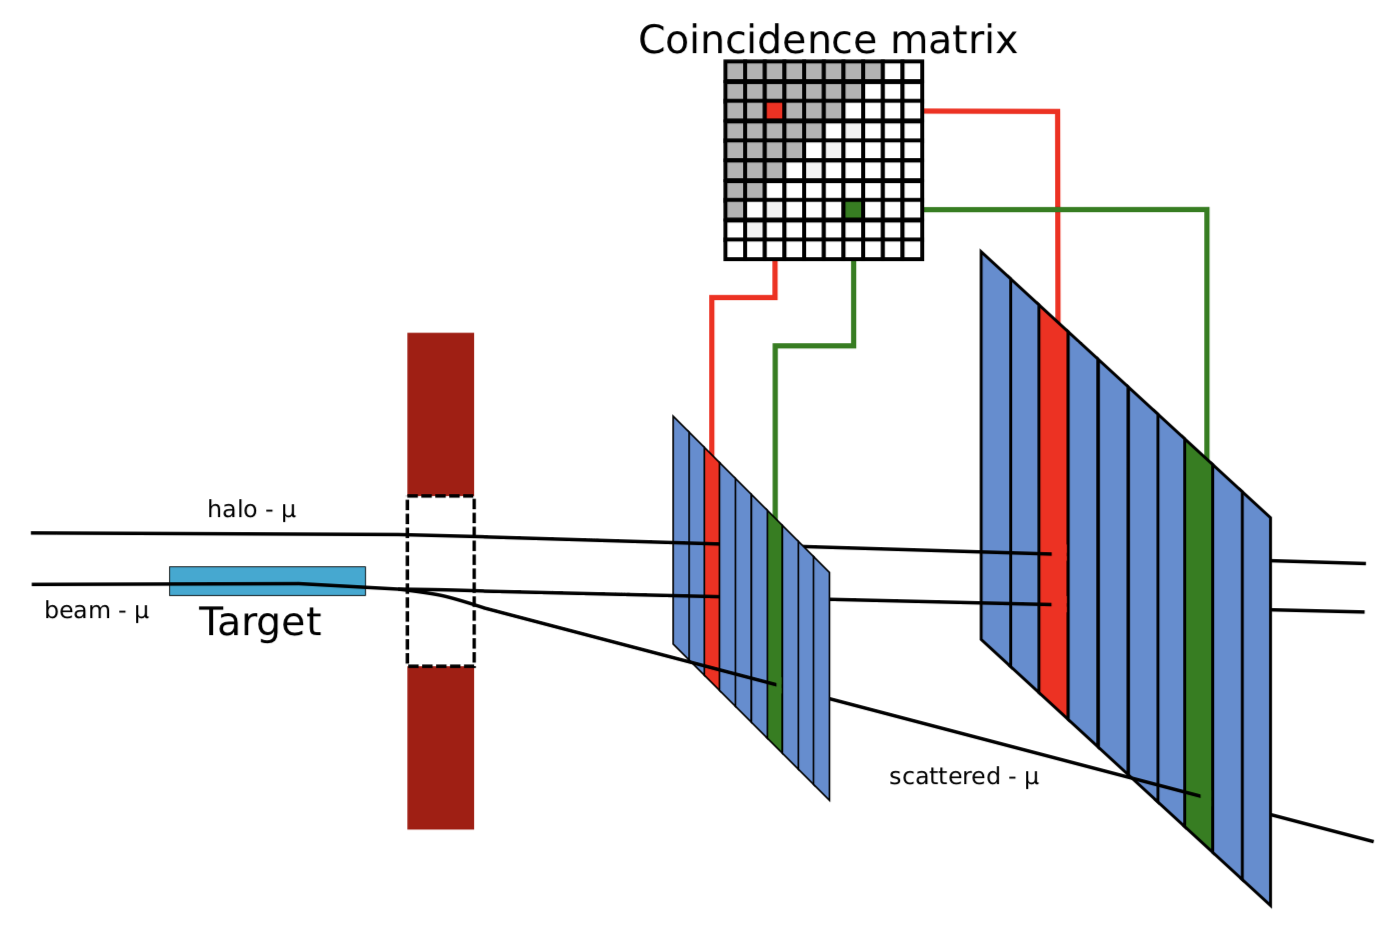
\includegraphics[scale=0.5]{./gfx/TriggerLogic.png}
	\caption{Concept of the trigger. The scattered muon leads to a coincidence in the activated area of the coincidence matrix while the halo muon fails to do so.}
	\label{pic:triglogic}
\end{figure}

The vertical component $\theta_y$ of the scattered muon is determined by using two hodoscopes with horizontal strips located at different positions along the beam direction. If $\theta_y$ is compatible with a vertex in the target position the trigger system validates the event. The $y$-$z$ plane is selected since the particle track is not deflected by the dipole magnet in $y$-direction. In cases where the scattering angle of the muon is too low to be measured ($Q^2 < 0.5$ (GeV/$c$)$^2$), the bending angle of the magnet is used to determine the momentum of the muon and thus trigger measures the energy loss relative to the beam energy.

The kinematic range covered by the trigger system is shown in Fig.~\ref{pic:trigger}. The trigger system is optimized to select DIS events. The lowest $Q^2$ events are covered by the \textit{ladder} trigger (LT) followed by \textit{middle} trigger (MT), \textit{outer} trigger (OT) and \textit{LAS} trigger (LAST) with increasing $Q^2$.

\begin{figure}[!h]
  \centering
	\subfloat[]{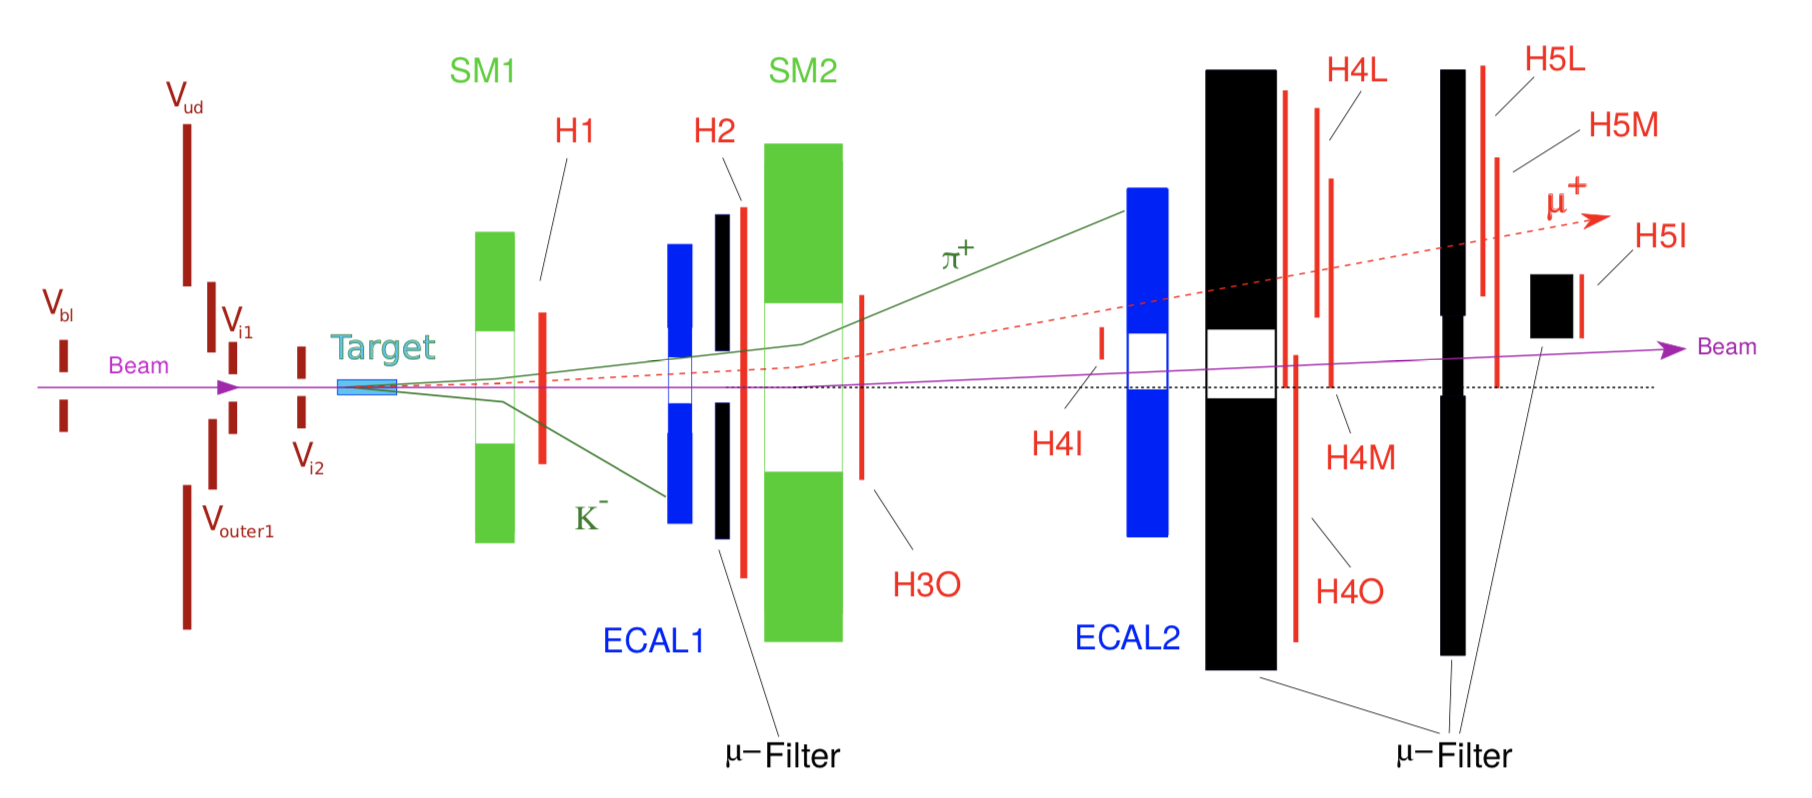
\includegraphics[scale=0.3]{./gfx/TriggerSys.png}}
  \subfloat[]{\includegraphics[scale=0.3]{./gfx/TriggerCov.png}}
	\caption{(a) Main elements of the trigger system. (b) Trigger system kinematic coverage.}
	\label{pic:trigger}
\end{figure}

%----------------------------------------------------------------------------------------

\section{Data Acquisition}

The data acquisition system (DAQ) \cite{NIM} is in charge of managing the information coming from more than $250000$ spectrometer electronic channels and building events. At COMPASS the typical event size is $45$ kB at a trigger rate of about $10$ kHz. The pipeline used in the DAQ is illustred in Fig.~\ref{pic:DAQ}. First the analog signals are coming from the detectors are preamplified if necessary, then they are digitized mostly directly at the front-end by Analog to Digital Converters (ADCs) or Time to Digital Converters (TDCs) according to the type of detectors the front-ends are coupled to. The data are then transferred to the readout driver modules CATCH (COMPASS Accumulate, Transfer and Control Hardware) of GeSiCA (GEM and Silicon Control and Acquisition) upon the arrival of a trigger signal provided by the Trigger Control System (TCS). CATCH and GeSiCA combine the data from up to $16$ cards (ADC or TDC) and transmit them via an optical S-Link to the computers named \textit{Readout Buffer} (ROBs, maximum through output 160 MB/s), where they are stored in $512$ MB spill buffer cards. During the $4.8$ s of a spill the data are written to memory, during the rest of the full SPS cycle ($36$ s) they are read through a PCI interface. In this way the required bandwidth is reduce by a factor of three. The events are built by 12 event builders and are then written to multiple $1$ GB large files (chunks) labeled by the run number and their consecutive chunk number. Finally the data are transferred to the CERN central data recording facility (CASTOR).

\begin{figure}[!h]
  \centering
	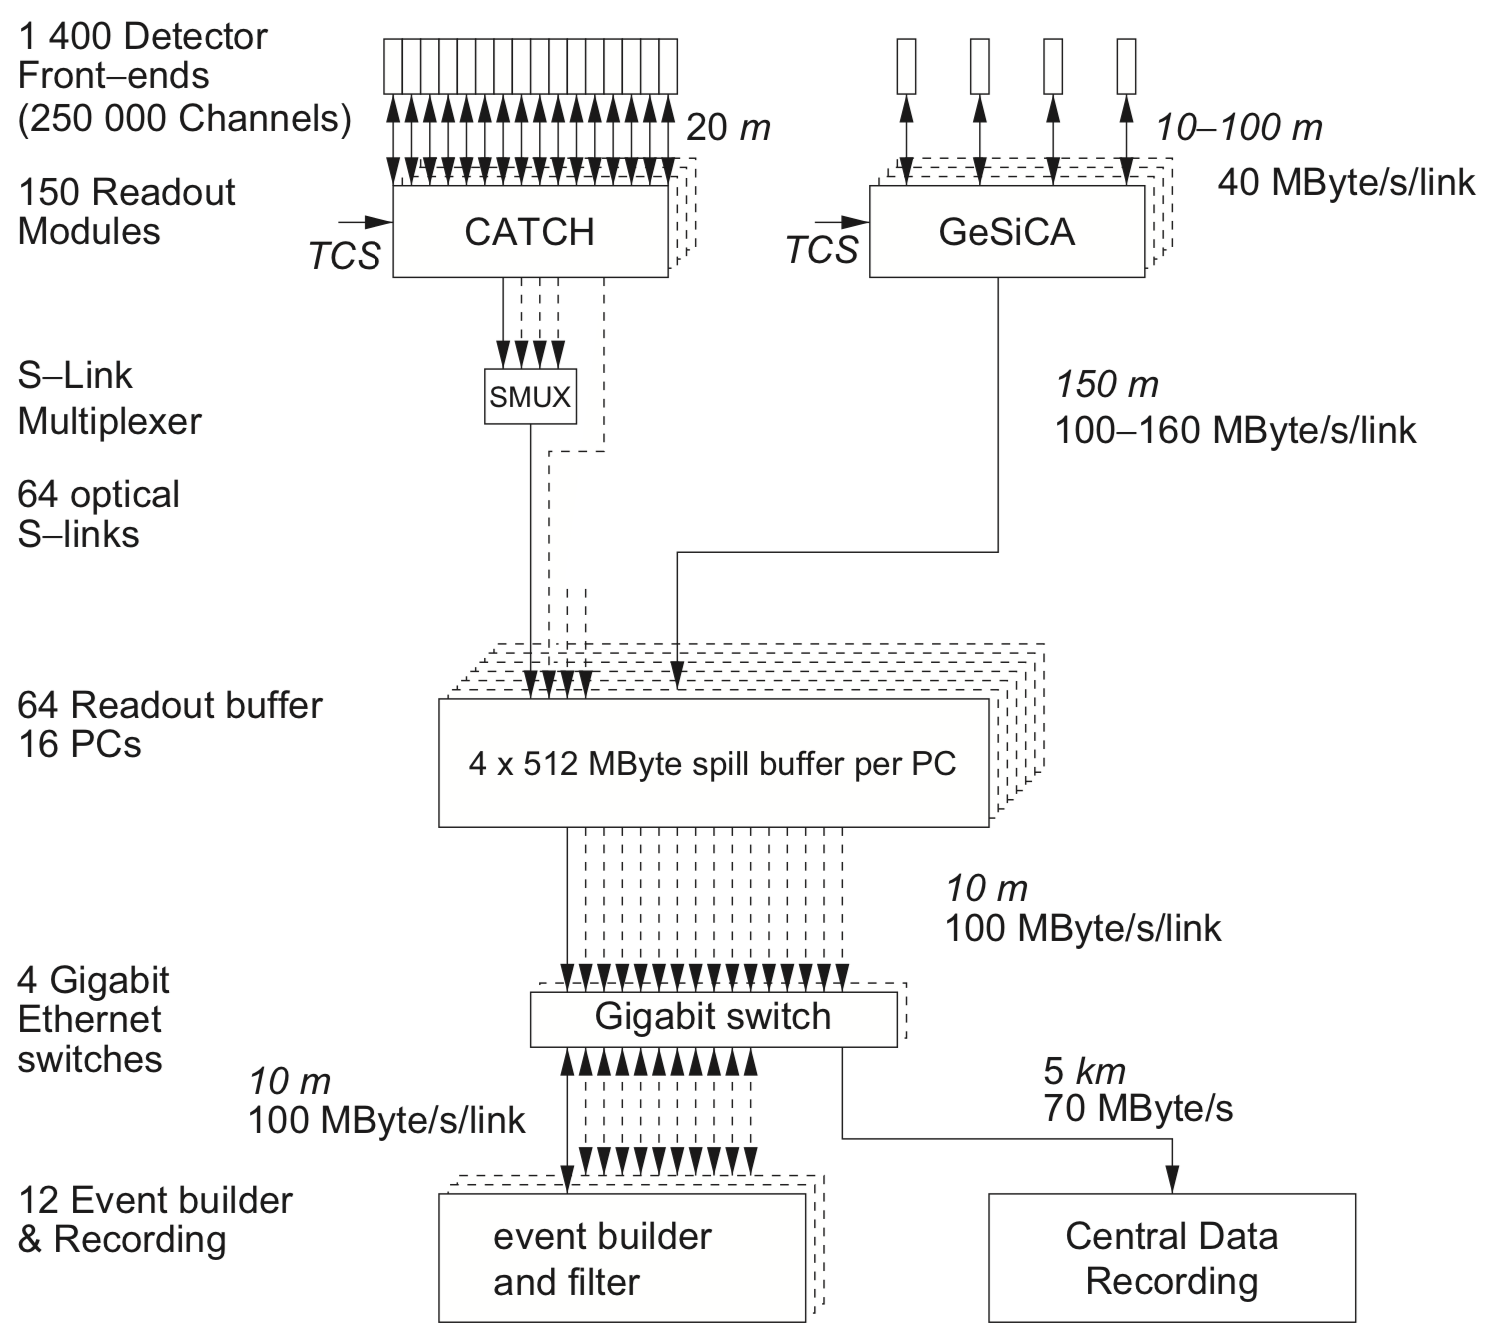
\includegraphics[scale=0.4]{./gfx/DAQ.png}
	\caption{General architecture of the DAQ system. Digitized data from the detector front-end are combined on the CATCH and GeSiCA modules. The storage of the data during the spill and the event building is performed locally. The data are recorded at the CERN computing center. Taken from \cite{NIM}.}
	\label{pic:DAQ}
\end{figure}

%----------------------------------------------------------------------------------------

\section{Event Reconstruction}

The offline reconstruction of the events stored in CASTOR is performed by the COMPASS software CORAL\footnote{COMPASS Reconstruction Algorithm Library} \cite{NIM}. CORAL is also used for the reconstruction of events generated by the Monte-Carlo simulation tool TGEANT (see Chapter~\ref{ch:MC}). CORAL is written in C++ and has a modular structure. The scheme of the steps followed by the reconstruction program is shown in Fig.~\ref{pic:CORAL}. First the information on the fired detectors channels is extracted. This is known as decoding and in the MC case digitization. In general there are more than one detector channels fired by the same particle. In that case a clustering algorithm is applied~:~the neighbouring detector channels that were fired are grouped together and the coordinate of the cluster in the apparatus reference system is computed. At this stage the detector calibration and position are used to extract the information. The CORAL output is stored in a ROOT Tree called mDST (mini Data Summary Tape).

The physics information is extracted from the mDST using the software package PHAST\footnote{PHysics Analysis Software Tools}. PHAST gives access to the reconstructed event information and it provides a set of algorithm to compute the relevant physics variables of each event. The PHAST outputs are stored again in a ROOT Tree. These files are significantly smaller than the mDSTs and are used for the final physics analysis.

In COMPASS, the experimental data are organized into several levels. The basic level are the events collected in one \textit{spill} provided by the SPS. A \textit{run} is the equivalent of $200$ spills. As there are machine development and/or realignment each week, the data are then structured in \textit{weeks} (also called \textit{period}) containing multiple runs.

\begin{figure}[!h]
  \centering
	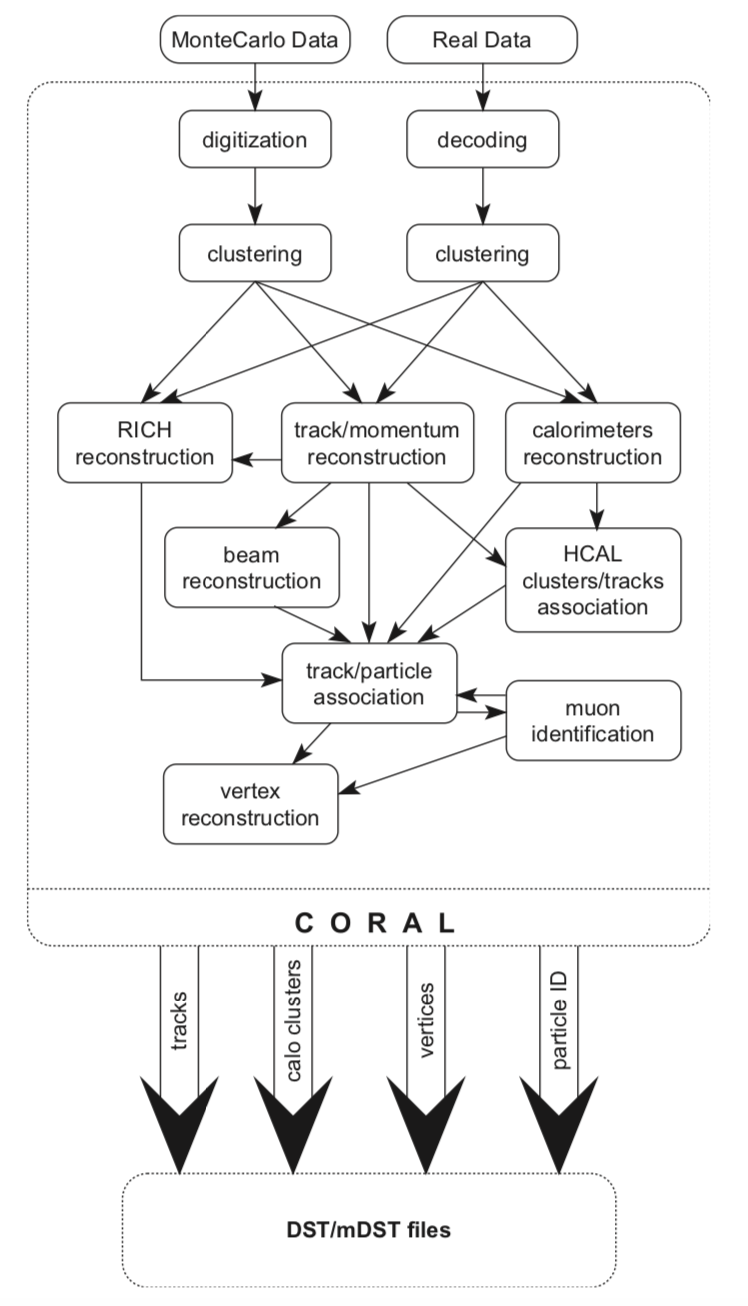
\includegraphics[scale=0.55]{./gfx/CORAL.png}
	\caption{Schematic representation of the COMPASS reconstruction software. Taken from \cite{NIM}.}
	\label{pic:CORAL}
\end{figure}
